\documentclass[tikz,border=2pt]{standalone}
\usepackage{pgfplots}
\usetikzlibrary{shapes.geometric, intersections}
\pgfplotsset{compat=1.7}

\begin{document}
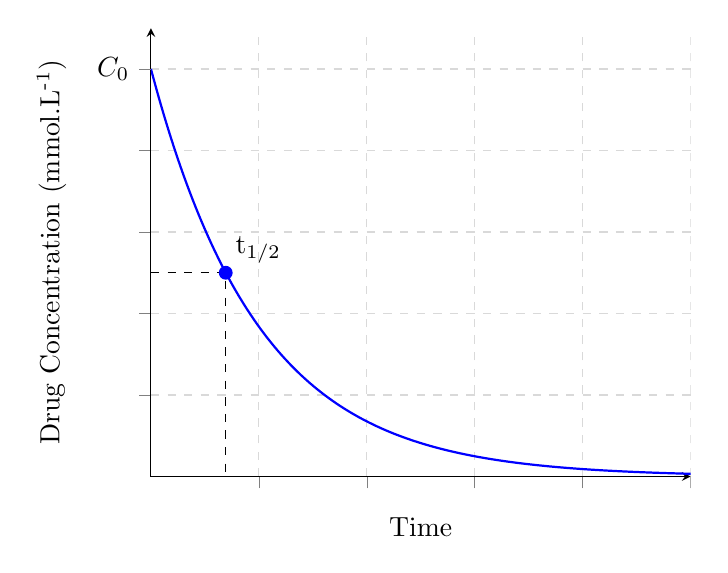
\begin{tikzpicture}

    \begin{axis}[
        axis x line=middle,
        axis y line=middle,
        x tick label style={/pgf/number format/fixed,
                            /pgf/number format/fixed zerofill,
                            /pgf/number format/precision=1},
        y tick label style={/pgf/number format/fixed,
                            /pgf/number format/fixed zerofill,
                            /pgf/number format/precision=0},
        grid = major,
        grid style={dashed, gray!30},
        xmin=0,     % start the diagram at this x-coordinate
        xmax= 5,    % end   the diagram at this x-coordinate
        ymin= 0,     % start the diagram at this y-coordinate
        ymax= 110,   % end   the diagram at this y-coordinate
        %axis background/.style={fill=white},
    	  x label style={at={(axis description cs:0.5,-0.1)},anchor=north},
	  y label style={at={(axis description cs:-0.1,.5)},rotate=90,anchor=south},
	  xticklabels={},
	 yticklabels={},
	extra y ticks={100},
extra y tick labels={$C_0$},
	 ylabel near ticks,
	xlabel near ticks,
        xlabel=Time,
        ylabel=Drug Concentration (mmol.L\textsuperscript{-1}),
        tick align=outside,
        enlargelimits=false]

	\addplot[domain=0:5, blue, thick,samples=500] {100*exp(-x))};

	\draw[black,thin,dashed] (axis cs: 0, 50) -- (axis cs: 0.693, 50) node[circle,fill=blue,inner sep=0pt,minimum size=5pt]{} node[above right]{t\textsubscript{1/2}} -- (axis cs: 0.693, 0);

\end{axis}

\end{tikzpicture} 
\end{document}